\documentclass[10pt,a4paper]{article}

%double si on veut une version prof et une version élève. simple si on veut une seule version.
\newcommand{\buildmode}{double}

\InputIfFileExists{version.tex}{}{}
% Version (définie par le script)
\providecommand{\version}{eleve}

\usepackage{feuilleexo}
\usepackage{schemaevolution}

%%%à modifier à chaque fois

\renewcommand{\niveau}{SBM 2A}
\renewcommand{\chapitre}{Fonctions exponentielle et logarithme}
\renewcommand{\numchap}{0.5} 
\renewcommand{\theme}{Fonctions}

\begin{document}


%\legendeicones

\vspace{-0.3cm}

\prof{
    \begin{itemize}
        \item Introduire le cours par des rappels. Dire qu'elle sert à résoudre des équations différentielles. Rappeler le graphique et les propriétés. Les faire noter si elles sont oubliées.
    \end{itemize}
}

\begin{prerequis}
\begin{itemize}        
        \item Savoir Résoudre une équation
        \item Savoir lire graphiquement les images et les antécédents d'une fonction.
        \item Savoir dériver une fonction et étudier ses variations.
\end{itemize}

\end{prerequis}


On rappelle les représentations graphiques des fonnctions exponentielle et logarithmé népérien :

\begin{multicols}{2}
    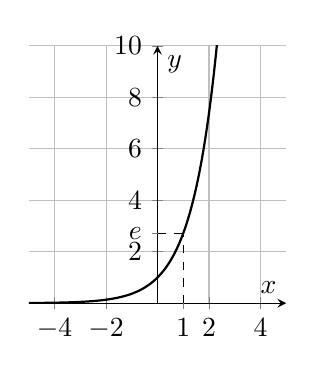
\begin{tikzpicture}
    \begin{axis}[
        axis lines = middle,
        xmin = -5,
        xmax = 5,
        ymin = 0,
        ymax = 10,
        width = 0.4\textwidth,
        height = 0.4\textwidth,
        grid = both,
        xlabel = \(x\),
        ylabel = \(y\),
        extra y ticks = {2.71828},
        extra y tick labels = {$e$},  
        extra y tick style = {grid = none},  
        extra x ticks = {1},
        extra x tick labels = {$1$},  
        extra x tick style = {grid = none},  
    ]
        \addplot[
            domain=-5:5,
            samples=200,
            thick
        ] {exp(x)};
        \addplot[
            dashed,
            domain=0:1
        ] {exp(1)};
        \addplot[
            dashed
        ] coordinates {(1,0) (1,e)};
    \end{axis}
\end{tikzpicture}

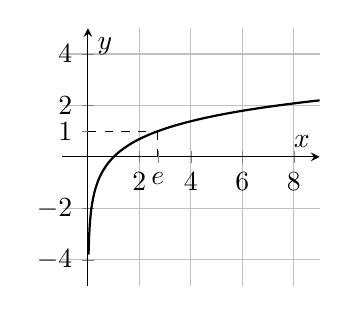
\begin{tikzpicture}
    \begin{axis}[
        axis lines = middle,
        xmin = -1,
        xmax = 9,
        ymin = -5,
        ymax = 5,
        width = 0.4\textwidth,
        height = 0.4\textwidth,
        grid = both,
        xlabel = \(x\),
        ylabel = \(y\),
        extra x ticks = {2.71828},
        extra x tick labels = {$e$},  
        extra x tick style = {grid = none},  
        extra y ticks = {1},
        extra y tick labels = {$1$},  
        extra y tick style = {grid = none},  
    ]
        \addplot[
            domain=0:9,
            samples=400,
            thick
        ] {ln(x)};
        \addplot[
            dashed,
            domain=0:e
        ] {1};
        \addplot[
            dashed
        ] coordinates {(e,0) (e,1)};
    \end{axis}
\end{tikzpicture}
\end{multicols}

\begin{multicols}{2}

    \section{Equations et résolutions graphiques}
    \begin{exo}[][]
        À l'aide des représentations graphiques des fonction \(exp\) et \(ln\), retrouver les valeurs suivantes :
        \begin{tasks}(2)
        \task \(\exp(0)\)
        \task \(\exp(1)\)
        \task \(\ln(1)\)
        \task \(\ln(e)\)
        \end{tasks}
    \end{exo}

    \begin{exo}[][]
        Résoudre les équations suivantes, et contrôler les résultats graphiquement :
        \begin{tasks}(2)
        \task \(e^x = 1\)
        \task \(e^x = e^{-1}\)
        \task \(e^x = -1\)
        \task \(e^x = 0\)
        \task \(\ln(x) = 1\)
        \task \(\ln(x) = 0\)
        \task \(\ln(x) = -1\)
        \task \(\ln(x) = -4\)
        \end{tasks}
    \end{exo}

    \begin{exo}[][]
        Résoudre les équations suivantes.
        \begin{tasks}(2)
        \task \(e^{x+2} = e^2\)
        \task \(e^{-x+2} = e\)
        \task \(7-e^{3x-1} = 0\)
        \task \(\ln(x) = \ln(3)\)
        \task \(\ln(x) -3 = 0\)
        \task \(\ln(3x+1) = 2\)
        \end{tasks}
    \end{exo}

\section{Dérivation et études de fonctions}

\begin{exo}[][]
    Dériver les fonctions suivantes :
    \begin{tasks}(2)
\task $f(x) = e^{3x+1}$
\task $g(x) = e^{x+2}$
\task $h(x) = -2e^{-4x}$
\task $h(x) = -2e^{-4x}+ 3x + \ln(x)$
\end{tasks}
\end{exo}

\begin{exo}[][]
    \begin{enumerate}
        \item Etudier les variations des fonctions suivantes :\begin{tasks}(2)
            \task $l(x)= e^{2x}$
            \task $m(x)= e^{-x}$
            \task $n(x)=  e^{\frac{1}{2}x}$
            \task $o(x)=  e^{-5x}$
        \end{tasks}
        \item Que remarquez-vous ?
    \end{enumerate}
\end{exo}

\begin{exo}[Inspiré de l'examen du 15 mai 2023][ccf]\\
Afin de vérifier la bonne isolation thermique d'un spa, on porte la température du spa à 38 degrés puis on coupe l'alimentation électrique du spa qui sert à faire chauffer l'eau. \\
On s'intéresse à l'évolution de cette température en fonction du temps écoulé à partir de cette coupure. \\
On modélise la température du spa en fonction du temps $t$, en heures par une fonction $f$ définie par $$
f(t) = 13e^{-0.05t}+25
$$
\begin{enumerate}
\item Quelle était la température initiale ?
\item Calculer la valeur arrondie à $10^{-1}$ de $f(24)$.\\
Interpréter cette valeur dans le contexte de l'exercice.
\item \begin{enumerate}
\item Pour tout réel $t$ de l'intervalle $[0;+\infty[$, déterminer une expression de $f'(t)$. 
\item En déduire le sens de variations de la fonction $f$ sur l'intervalle $[0;+\infty[$.
\item Ce sens de variations vous paraît-il cohérent avec le contexte de l'exercice ? Argumentez.
\end{enumerate}
\end{enumerate}
\end{exo}

\begin{exo}[][appro]
On considère les fonctions suivantes, toutes définies sur $\R$ :
\begin{tasks}(2)
\task $f(x) = e^{2x}$
\task $g(x) = e^{-2x}$
\task $h(x) = -e^{2x}$
\task $i(x) = -e^{-2x}$
\end{tasks}
Faire correspondre chacune de ces représentation à leur courbe :\begin{tasks}(2)
\task \begin{tikzpicture}[scale=0.8]
\clip (-2,-2) rectangle (2,2);
\draw (-2,0) -- (2,0);
\draw (0,-2) -- (0,2);
\draw[color=blue, domain=-2:1]   plot (\x,{exp(2*\x)})    node[pos=-1,below left] {$\mathcal{C}_1$};
\draw (0.1,1)--(-0.1,1) node[left] {1};
\end{tikzpicture}
\task \begin{tikzpicture}[scale=0.8]
\clip (-2,-2) rectangle (2,2);
\draw (-2,0) -- (2,0);
\draw (0,-2) -- (0,2);
\draw[color=blue, domain=-2:1]   plot (\x,{-exp(2*\x)})    node[pos=0.01,below left] {$\mathcal{C}_2$};
\draw (-0.1,-1)--(0.1,-1) node[right] {-1};
\end{tikzpicture}
\task \begin{tikzpicture}[scale=0.8]
\clip (-2,-2) rectangle (2,2);
\draw (-2,0) -- (2,0);
\draw (0,-2) -- (0,2);
\draw[color=blue, domain=-0.5:2]   plot (\x,{-exp(-2*\x)})    node[pos=0.95,above right] {$\mathcal{C}_3$};
\draw (-0.1,-1)--(0.1,-1) node[right] {-1};
\end{tikzpicture}
\task \begin{tikzpicture}[scale=0.8]
\clip (-2,-2) rectangle (2,2);
\draw (-2,0) -- (2,0);
\draw (0,-2) -- (0,2);
\draw[color=blue, domain=-1:2]   plot (\x,{exp(-2*\x)})    node[pos=0.95,above right] {$\mathcal{C}_4$};
\draw (0.1,1)--(-0.1,1) node[left] {1};
\end{tikzpicture}
\end{tasks}
\end{exo}


\end{multicols}
\end{document}
